\documentclass[11pt, a4paper, twoside]{article}
\usepackage[utf8x]{inputenc}
\usepackage[spanish]{babel}
\usepackage{times}
\usepackage[T1]{fontenc}
\usepackage{anysize}
\usepackage{tabu}
\usepackage{pdfpages}
\usepackage{fancyhdr}

% Penaliza los guiones a final de línea
\hyphenpenalty = 9999

\marginsize{3cm}{2cm}{2cm}{2cm}

% Indicador completo en lugar de página
\fancyhead[LR]{}
\fancyfoot[C]{{\ttfamily RTF CT:PRSGR \quad \thepage}}

\renewcommand*{\headrulewidth}{0pt}
\pagestyle{fancy}

\renewcommand*{\appendix}{\setcounter{section}{0}\setcounter{subsection}{0}\renewcommand*{\thesection}{Anexo \Alph{section}}}

% Comando para indicar los problemas
\newcommand{\problema}[2]{\begin{description} \item[Exposición] #1 \item[Resolución] #2 \end{description}}

% Comando con el nombre del grupo revisado
\newcommand*{\Cauchy}{\mbox{\textsc{Cauchy-Team}} }

\begin{document}

	% Título
	\begin{center}
		\scshape \large Acta de la Revisión Técnica Formal \textit{Plan de Reducción, Supervisión y Gestión del Riesgo} - \Cauchy
	\end{center}

	Reunidos de una parte Daniel Báscones Garcia y Iñigo Zunzunegui Monterrubio en representación de\break \Cauchy en calidad de autores del documento y de la otra Sandra Bermejo Cañadas, Juan Andrés Claramunt Pérez y Rubén Rafael Rubio Cuellar de la parte revisora, el \textsc{Grupo Diedral}, se procede a la puesta en común de la Revisión Técnica Formal del documento \textsc{Plan de Reducción, Supervisión y Gestión del Riesgo} perteneciente a \Cauchy. \\

	El equipo revisor presenta un documento, anexo al presente, con sus conclusiones previas.\break \Cauchy defiende su documento y el \textsc{Grupo Diedral} expone los problemas encontrados, citados en dicho documento. Por lo cual el equipo revisor concluye:

\begin{quotation} \itshape
	El documento presenta una estructura general correcta, con pequeños problemas de formato como la falta de versión en la cabecera o los margenes de alguna tabla. En la reunión realizada se acuerda la revisión de la valoración de algunos de los riesgos y considerar la inclusión de otros. Se señala también la falta de nombres en portada, algo fácilmente subsanable.
\end{quotation}

\noindent
En virtud de lo anterior, el documento se declara \textsc{aceptado}.\\

	Ambas partes expresan su conformidad con lo referido en este acta en Madrid, a \today.

\begin{flushleft}
	Los asistentes,
\end{flushleft}

\vspace{1cm}

	% Espacio para firmar
	\begin{tabu} to .9\linewidth {X[1,c] X[1, c]}
		Daniel Báscones Garcia & Iñigo Zunzunegui Monterrubio
	\end{tabu}

	\vfill

	\begin{tabu} to .9\linewidth {X[1,c] X[1, c]}
		Sandra Bermejo Cañadas & Juan Andrés Claramunt Pérez & Rubén Rafael Rubio
	\end{tabu}
	
	\vfill
	{\itshape A continuación se incluye el anexo previo elaborado por el equipo revisor: }

	% Incluye el anexo del otro grupo
	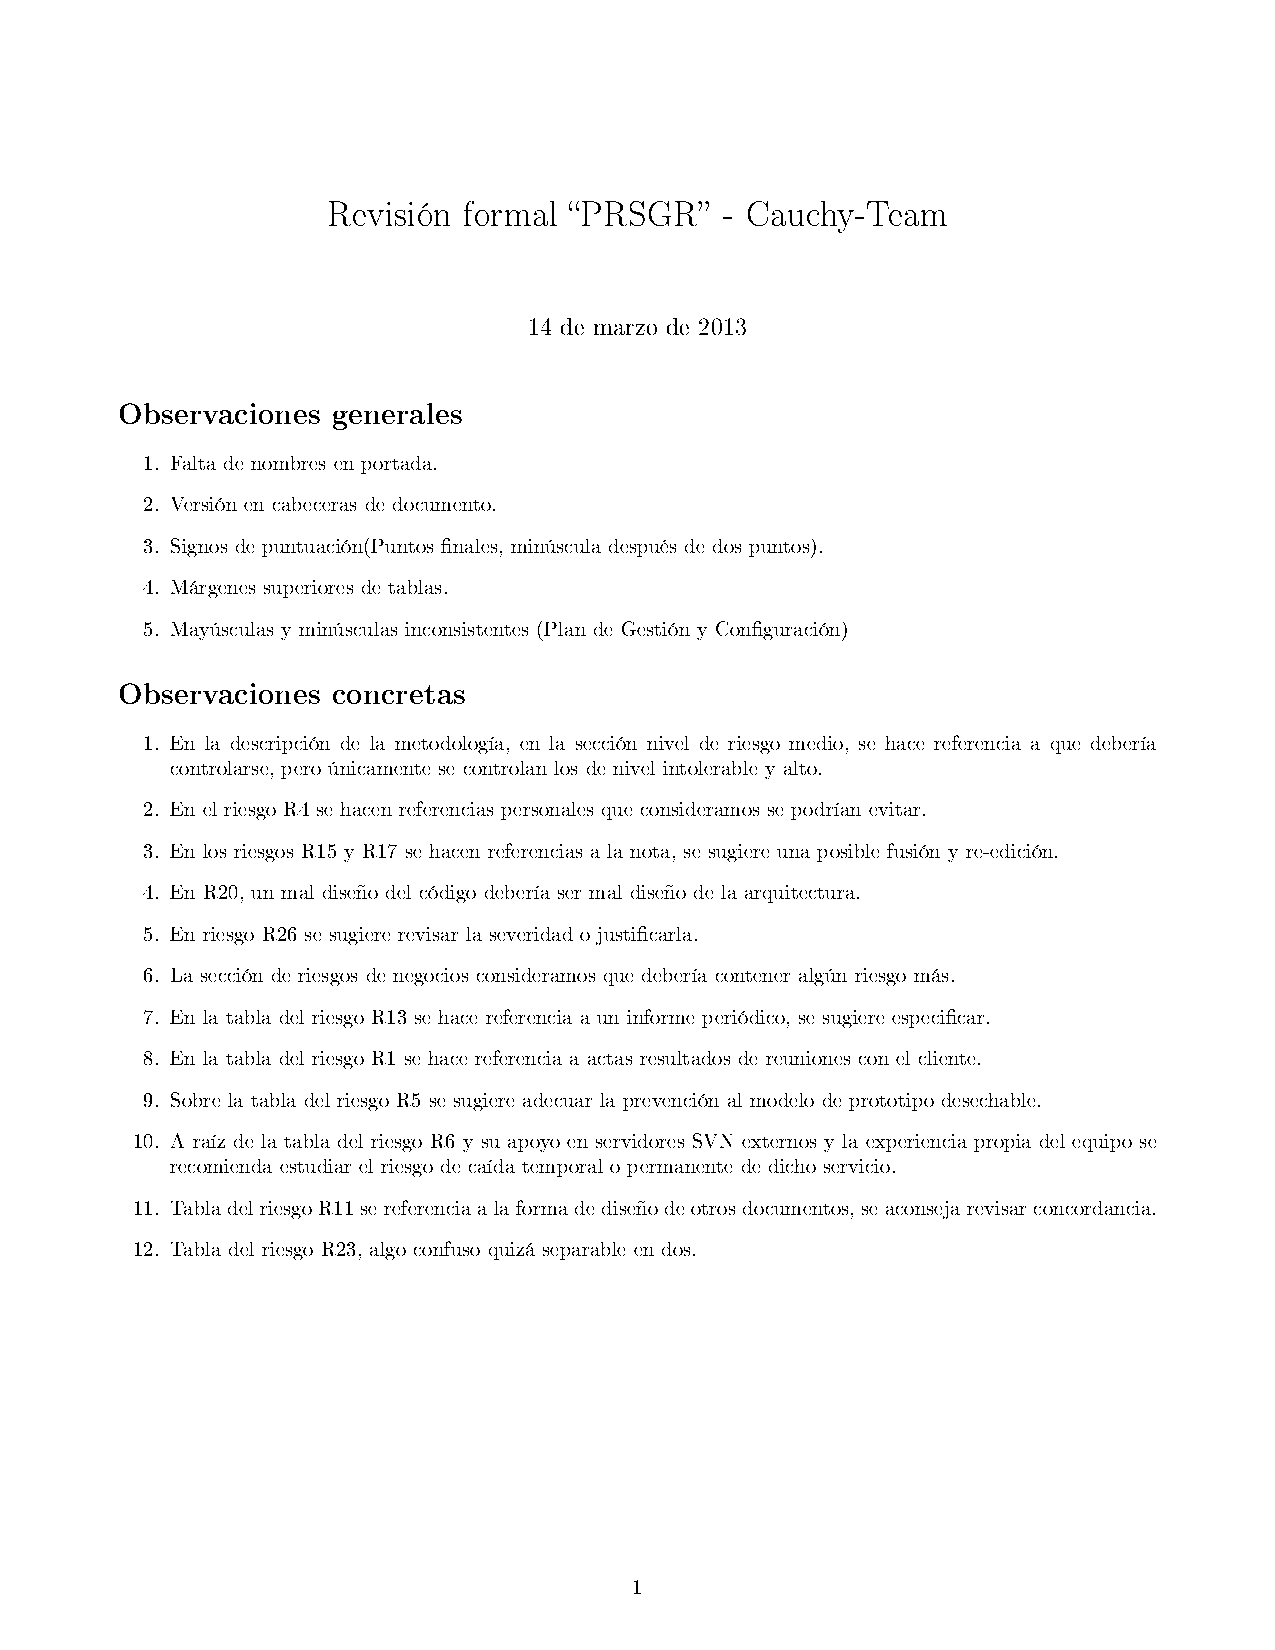
\includepdf[pages=1-2, pagecommand={}]{riesgos_cauchy_anexo.pdf}
\end{document}
